% !TEX root = exam.tex
\ifthenelse{\equal{\type}{booklet}}{
\newcommand{\GMMkMeansStudSolA}{
%%%%%%%%%%%%%%%%%%%%%%%%%%%%%%%%%%%%
%%
%%.   YOUR SOLUTION FOR PROBLEM A BELOW THIS COMMENT
%%
%%%%%%%%%%%%%%%%%%%%%%%%%%%%%%%%%%%%
\vspace{2.5cm}
}

\newcommand{\GMMkMeansStudSolB}{
%%%%%%%%%%%%%%%%%%%%%%%%%%%%%%%%%%%%
%%
%%.   YOUR SOLUTION FOR PROBLEM A BELOW THIS COMMENT
%%
%%%%%%%%%%%%%%%%%%%%%%%%%%%%%%%%%%%%
\vspace{3cm}
}

\newcommand{\GMMkMeansStudSolC}{
%%%%%%%%%%%%%%%%%%%%%%%%%%%%%%%%%%%%
%%
%%.   YOUR SOLUTION FOR PROBLEM A BELOW THIS COMMENT
%%
%%%%%%%%%%%%%%%%%%%%%%%%%%%%%%%%%%%%
\vspace{2.5cm}
}

\newcommand{\GMMkMeansStudSolD}{
%%%%%%%%%%%%%%%%%%%%%%%%%%%%%%%%%%%%
%%
%%.   YOUR SOLUTION FOR PROBLEM A BELOW THIS COMMENT
%%
%%%%%%%%%%%%%%%%%%%%%%%%%%%%%%%%%%%%
\vspace{2cm}
}

\newcommand{\GMMkMeansStudSolE}{
%%%%%%%%%%%%%%%%%%%%%%%%%%%%%%%%%%%%
%%
%%.   YOUR SOLUTION FOR PROBLEM A BELOW THIS COMMENT
%%
%%%%%%%%%%%%%%%%%%%%%%%%%%%%%%%%%%%%
\vspace{3cm}
}

%\newcommand{\GMMkMeansStudSolF}{
%%%%%%%%%%%%%%%%%%%%%%%%%%%%%%%%%%%%%
%%%
%%%.   YOUR SOLUTION FOR PROBLEM A BELOW THIS COMMENT
%%%
%%%%%%%%%%%%%%%%%%%%%%%%%%%%%%%%%%%%%
%\vspace{12cm}
%}
 %The students have to fill this file to print the solution
}{
\input{GMMkMeans_OurSolution} %This file will not be provided to students since it contains the solution
}

% Problem Explanation:
% - first argument is the number of points
% - second argument is the title and the text
\examproblem{10}{K-Means\\}


%%%%%%%%%%%%%%%%%%%%%%%%%%%%%%%%%%%%%%
%%%%%  BEGINNING OF SUBPROBLEMS LIST

\begin{enumerate}

 % Subproblem description
\examproblempart{Mention if K-Means is a supervised or an un-supervised method.
 \\}

\bookletskip{0.0}   %in inches

% Solution box
 \framebox[14.7cm][l]{
 \begin{minipage}[b]{14.7cm}
 \inbooklet{Your answer: \GMMkMeansStudSolA}
  
 \solution{\GMMkMeansSolA}
 \end{minipage}
 }
 
  % Subproblem description
\examproblempart{Assume that you are trying to cluster data points $x_{i}$  for $ i \in \{1,2 \dots D\}$ into K clusters each with center $\mu_{k}$  where $ k \in \{1,2, \dots K \}$. The objective function for doing this clustering involves minimizig the euclidean distance between the points and the cluster centers. It is given by  \begin{equation*}
\min\limits_{\mu} \min\limits_{r}\sum\limits_{i \in D} \sum\limits_{k =1}^{K} \frac{1}{2} r_{ik} ||x_{i} -\mu_{k}||_{2}^{2} \\
 \end{equation*} \\ How do you ensure hard assignemnt of one data point to one and only one cluster at a given time? Note: By hard assignment we mean that your are 100 \% sure that a point either belongs or not belongs to a cluster.\\}

\bookletskip{0.0}   %in inches

% Solution box
 \framebox[14.7cm][l]{
 \begin{minipage}[b]{14.7cm}
 \inbooklet{Your answer: \GMMkMeansStudSolB}
  
 \solution{\GMMkMeansSolB }
 \end{minipage}
 }
 
% Subproblem description
\examproblempart{What changes must you do in your answer of part b, to make the hard assingment into a soft assignment? Note: By soft assignment we mean that your are  sure that a point either belongs or not belongs to a cluster with some probability.\\}

\bookletskip{0.0}   %in inches

% Solution box
 \framebox[14.7cm][l]{
 \begin{minipage}[b]{14.7cm}
 \inbooklet{Your answer: \GMMkMeansStudSolC}
  
 \solution{\GMMkMeansSolC}
 \end{minipage}
 }
 
 % Subproblem description
 \examproblempart{Looking at the following plot, what is the best choice for number of clusters?}
  \begin{center}
 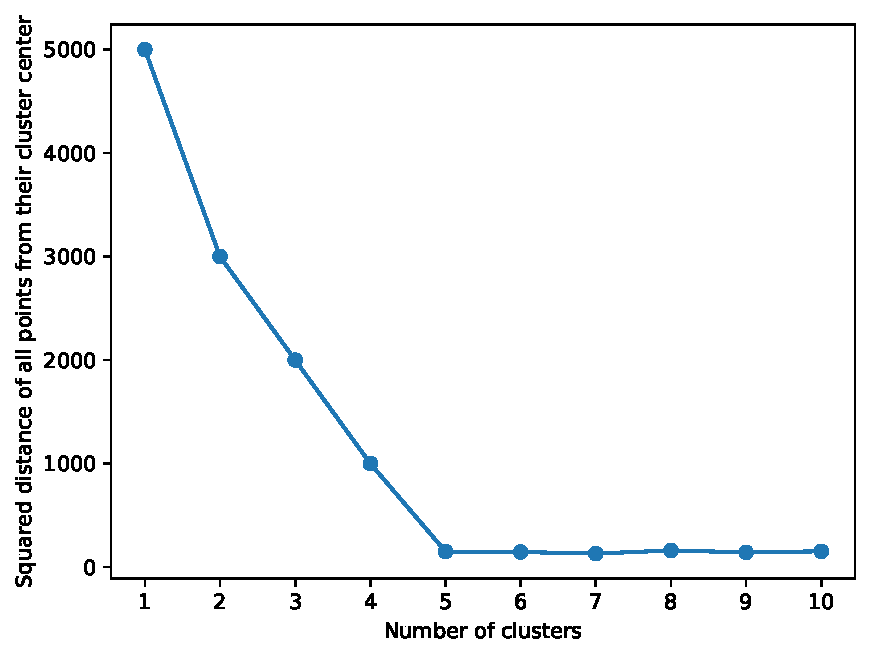
\includegraphics[width=8cm]{fig/cluster.pdf}
 \end{center}
\bookletskip{0.0}   %in inches

% Solution box
 \framebox[14.7cm][l]{
 \begin{minipage}[b]{14.7cm}
 \inbooklet{Your answer: \GMMkMeansStudSolD}
  
 \solution{\GMMkMeansSolD}
 \end{minipage}
 }

% Subproblem description
 \examproblempart{Would K-Means be an effecient algorithm to cluster the following data? Explain your answer in a couple of lines.}
  \begin{center}
 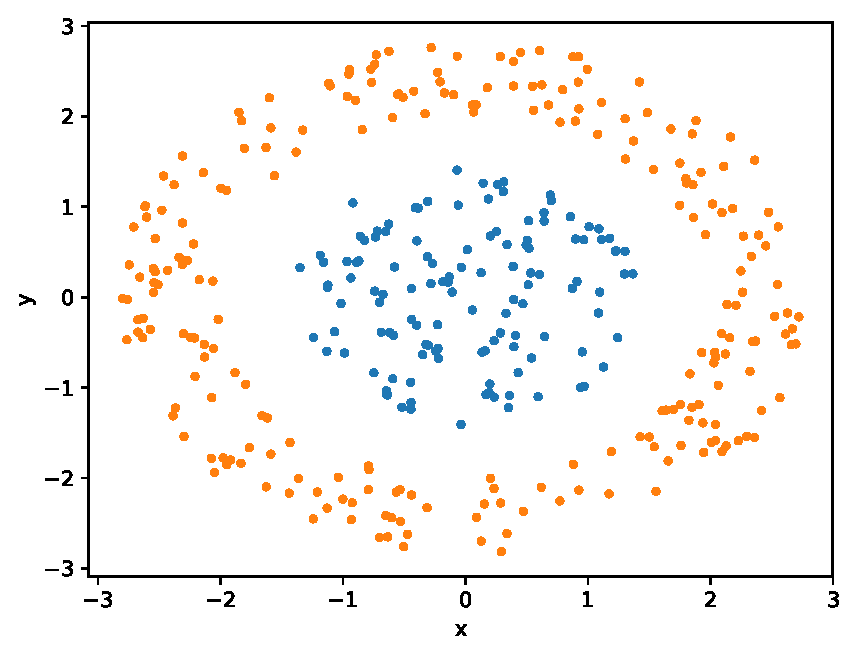
\includegraphics[width=8cm]{fig/concentric.pdf}
 \end{center}
\bookletskip{0.0}   %in inches

% Solution box
 \framebox[14.7cm][l]{
 \begin{minipage}[b]{14.7cm}
 \inbooklet{Your answer: \GMMkMeansStudSolE}
  
 \solution{\GMMkMeansSolE}
 \end{minipage}
 }
 
 %}
 
  %%%%%%%%%%%% END OF SUBPROBLEMS LIST
  
 \end{enumerate}